%!TEX root = ../dissertation.tex
% this file is called up by thesis.tex
% content in this file will be fed into the main document

%: ----------------------- introduction file header -----------------------
% the code below specifies where the figures are stored
\graphicspath{{3-mir/figures/}}

\chapter{Music Information Retrieval for Transcription}
\label{ch:mir}

Being able to accurately identify all musical events from audio and transcribe them into musical notations is an essential skill for musicians as well as a paramount goal of music machine learning research.
Enabling an automatic conversion from musical audio to symbolic notations, and vice versa through music synthesis, opens up many new possibilities.
The most straightforward application of automatic music transcription would be a software tool that transcribes audio recording and produces a musical score, which can aid musicians in various situations.
Automatic music transcription can help build a melody database to be used for music retrieval systems, such as query by humming \cite{molina2014humming}, where it is often very hard to obtain annotated data even when the audio files are abundantly available.
Similarly, by building a database containing symbolic information of music, music recommender systems can leverage the database to infer how much individual users would prefer the music, based on melodic, harmonic, and instrumental information present in the transcription.

As stated, due to the complexity and difficulty of creating an all-encompassing end-to-end music transcription system, many existing approaches focus on a specific subtask of the problem \cite{casey2008mir}, e.g. extracting onsets and beats, recognizing timbre and instruments, tracking monophonic and polyphonic pitches, or separating audio sources from a mixture.
Each of these subtasks poses interesting goals and applications even without the lofty goal of the full music transcription, and they are often classified under the umbrella term of music information retrieval (MIR).
Although this term has existed since 1960s \cite{kassler1966mir}, it was only after the late 1990s when active research on this area has spun off from computer music and computational musicology literature.
During the last two decades, numerous sophisticated and novel approaches for each of these subproblems have been introduced, that have continuously improved the performance in terms of the accuracy in predicting the correct annotations.
This chapter will first introduce the standard pipeline of music information retrieval, followed by a few state-of-the-art techniques for music transcription.

\section{The Standard Pipeline}

Audio data is huge in volume --- a typical audio track contains 44,100 real-numbered samples per second, and sometimes even more.
Therefore, computational methods for extracting musical information from audio usually contains a pipeline of feature extraction stages to reduce the volume and increase the interpretability of input data, as shown in Figure \ref{fig:pipeline}.
The pipeline shares many techniques that have been widely used in speech processing, but also many feature extraction stages are created for music-specific purposes.

\begin{figure}[t]
	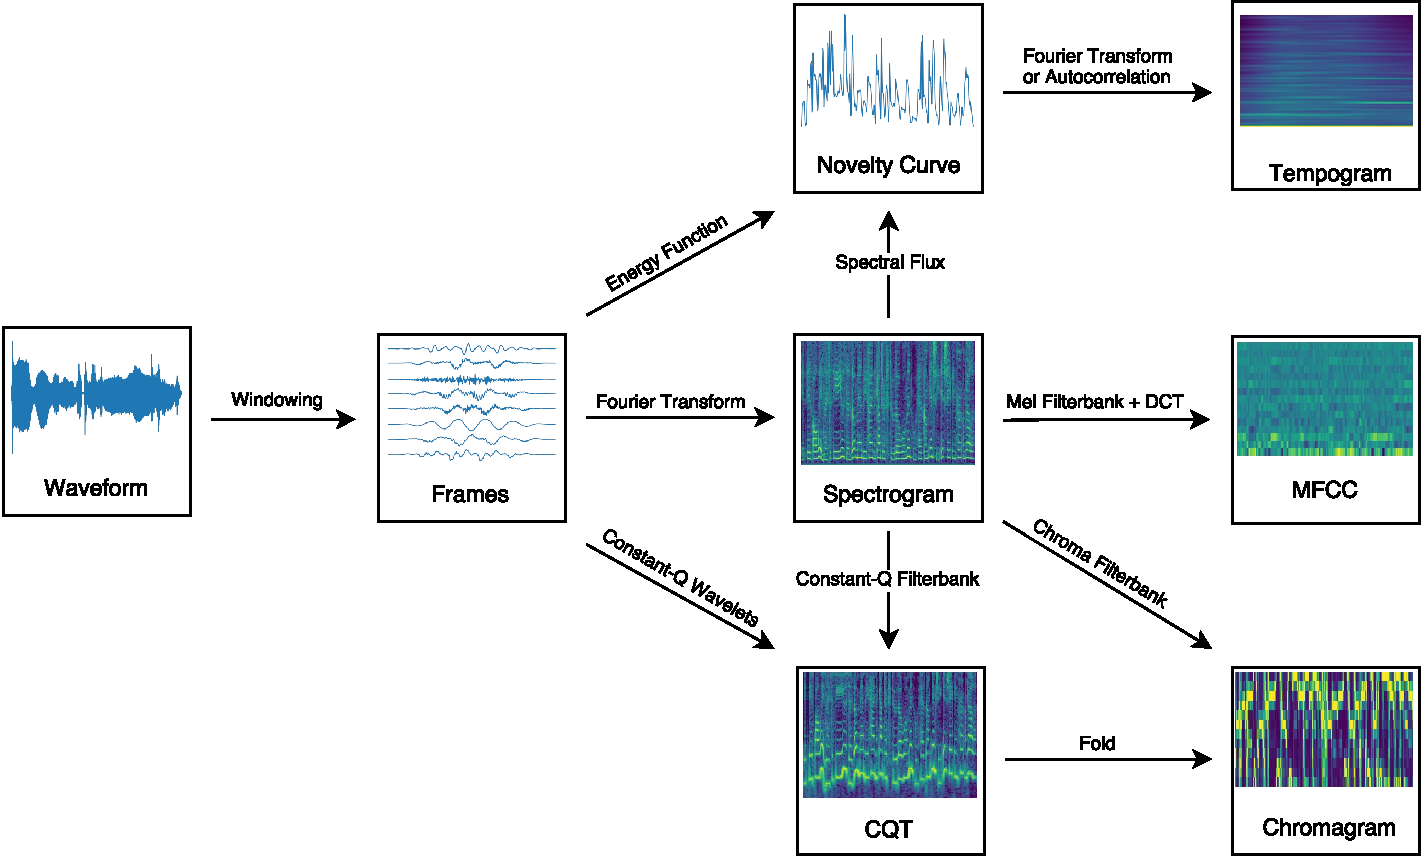
\includegraphics[width=\textwidth]{pipeline.pdf}
	\caption{\small The standard pipeline for music feature extraction. An appropriate set of feature extraction methods needs to be heuristically selected depending on the task.}\label{fig:pipeline}
\end{figure}

While there are many MIR tasks that operate on the track-level, such as music recommendation, tagging, and genre classification, most subtasks of music transcription involve the prediction of labels that are dependent on time, operating either in the sample-level or frame-level.
Frames are created by taking a series of overlapping short-time audio segments, where the length of a segment is typically 10-50 milliseconds, and optionally multiplying them by a windowing function.
Taking discrete Fourier transforms on the frames produces a short-time Fourier transform (STFT), and the magnitude of an STFT gives a spectrogram.
Spectrograms give very rich information about the audio; for example, the contour of melodies and dynamics of music are usually identifiable from the image.
However, the dimensionality of a spectrogram is still quite high, making it computationally prohibitive to run many algorithms directly on an STFT or a spectrogram.
This necessitated further transformations by the means of filterbanks, producing Mel-Frequency Cepstral Coefficients (MFCC) via the Mel filterbank, or chroma features by applying 12 filters specific to each scale degree.
Constant-Q transform (CQT) \cite{schorkhuber2010cqt} alleviates a drawback of STFT in which the linear spacing of frequency bins does not align with human auditory perception, by placing the center frequencies of filters to have a constant Q factor, which is the ratio between the center frequency and the 3 dB bandwidth of a filter.
By configuring CQT to produce 12 filters per octave, it is possible to obtain the coefficients corresponding to each musical tone, and to fold the representation to produce a chroma feature.
To extract the beat and tempo information, heuristic functions like the first-order difference of the time-domain log energy function or the spectral flux that measures the total energy increase over the frequency bins, to formulate a novelty curve, which measures energy bursts typically present in the onsets of notes.
The onset information can then be further processed to obtain tempo information via tempograms.


%Although a few recent techniques were successfully applied on the raw audio data without a predefined feature transformation,

While the pipeline shown in Figure \ref{fig:pipeline} is considered a de-facto standard for any audio processing systems, recent deep learning approaches have successfully eliminated some or all feature transformation stages by training model to learn the feature from the spectrogram or audio waveforms.
In theory, any feature extraction stage induces a loss of information, and it suggests that the best-performing model would benefit most from the raw audio data.

\section{Multiple Fundamental Frequency Estimation}

Among the aforementioned subtasks of automatic music transcription, estimating the pitch from polyphonic recording poses the most difficult challenges, as apparent from the recent stream of results from MIREX challenges \cite{downie2014mirex}.
The task is commonly referred to as multiple fundamental frequency estimation (Multi-F0 estimation, or MFFE), and in some sense supersedes the onset and beat detection problems as well as chord and melody tracking problems,
since the frequency tracking has to indicate the onset and offset of every sound, and tracking chords and melodies becomes much easier when the correct annotations for all pitch contours are available.

Many early methods for MFFE \cite{klapuri2003multiple,emiya2010multipitch} focused on extracting features like harmonicity and spectral smoothness from the audio spectrogram and devising a good heuristic for frequency estimation.
More recent models employ data-driven approaches, using dynamic Bayesian networks \cite{raczynski2013dynamic} or recurrent neural networks \cite{sigtia2016endtoend}, and achieved better performance.

The idea of using generative models to predict multiple fundamental frequencies is not new \cite{dubois2005harmonic,cemgil2006generative}, but they relied on manually designed generative models for sound generation, which might have led to poor generalizability.
Using deep generative models is expected to help overcoming this limitation, since deep learning methods is known to be excellent in learning embeddings and manifolds that are generalizable to different tasks and domains.



